\documentclass[conference]{IEEEtran}
\usepackage{graphicx}
\usepackage{amsmath}
\usepackage{booktabs}
\usepackage{cite}
\usepackage{url}
\graphicspath{{figures/}}

\begin{document}

\title{Multimodal Concealed Phone Detection}

% TODO: add every team member and check names/emails
\author{\IEEEauthorblockN{Yung-Hsin (Sean) Tsai}
\IEEEauthorblockA{Department of Electrical and Computer Engineering\\
Rice University, Houston, TX, USA\\
yt66@rice.edu}}

\maketitle

\begin{abstract}
Secure facilities need a way to find phones carried on a person without a pat-down. We are building a stand-off detector that combines a 300--330\,GHz FMCW imaging radar with an Intel RealSense D415 RGB-D camera. The radar produces a 3D point cloud of the body, and a PointNet++ network labels each radar point as phone or body. The calibrated camera crops the body from the scene and provides ground-truth phone labels automatically. In a pilot study with phones taped to a mannequin at 2.5--3.5\,m, phone points were not brighter than the body, so detection must rely on local shape. On held-out scans, the network found all six test phones with a mean centroid error of 5.8\,cm and a pooled phone IoU of 0.34, but five of seven test scans contained false alarms. We outline how more data and targeted training will reduce these errors.
\end{abstract}

\section{Introduction}
Personal phones are restricted in many secure locations, yet current screening relies on walk-through metal detectors and manual searches, which are slow and intrusive. Millimeter-wave body scanners image objects through clothing \cite{sheen2001}, and learned detectors have been applied to millimeter-wave and terahertz security images \cite{meng2020,pang2020}. Low-cost radar and sensor-fusion systems have also been used to detect concealed metal objects \cite{mitchell2023,kaul2024}. These systems either require the subject to stand inside a portal or report only whether an object is present.

Our goal is to locate a phone directly on the body from a distance. A phone is a rigid, flat rectangle with sharp edges, so a high-resolution 300\,GHz imaging radar should resolve its outline on the body surface. We treat the radar output as a 3D point cloud and segment it point by point with PointNet++ \cite{qi2017pointnetpp}, which extends PointNet \cite{qi2017pointnet} with local neighborhoods at several scales. An RGB-D camera, calibrated to the radar, isolates the body and provides automatic ground truth.

The project has three tasks: (1) build a labeled dataset with an automatic labeling pipeline; (2) train a PointNet++ phone segmenter and reach a held-out phone IoU of at least 0.5 with a detection rate of at least 95\%; and (3) evaluate phones concealed under clothing and next to distractors such as keys and belts. This report covers the method and partial results for tasks 1 and 2.

\section{Methods}

\subsection{Sensing System}
The system (Fig.~\ref{fig:setup}) consists of a 300--330\,GHz FMCW radar with mechanical beam steering over a $50^\circ\times30^\circ$ (azimuth $\times$ elevation) field of view and an Intel RealSense D415 RGB-D camera mounted below it. The two sensors are related by a rigid transform from our existing radar--camera calibration, with an additional azimuth correction. The radar's range resolution is about 30\,cm, which is larger than the thickness of a phone, so the phone and the body behind it fall in the same range bin.

\begin{figure}[t]
\centering
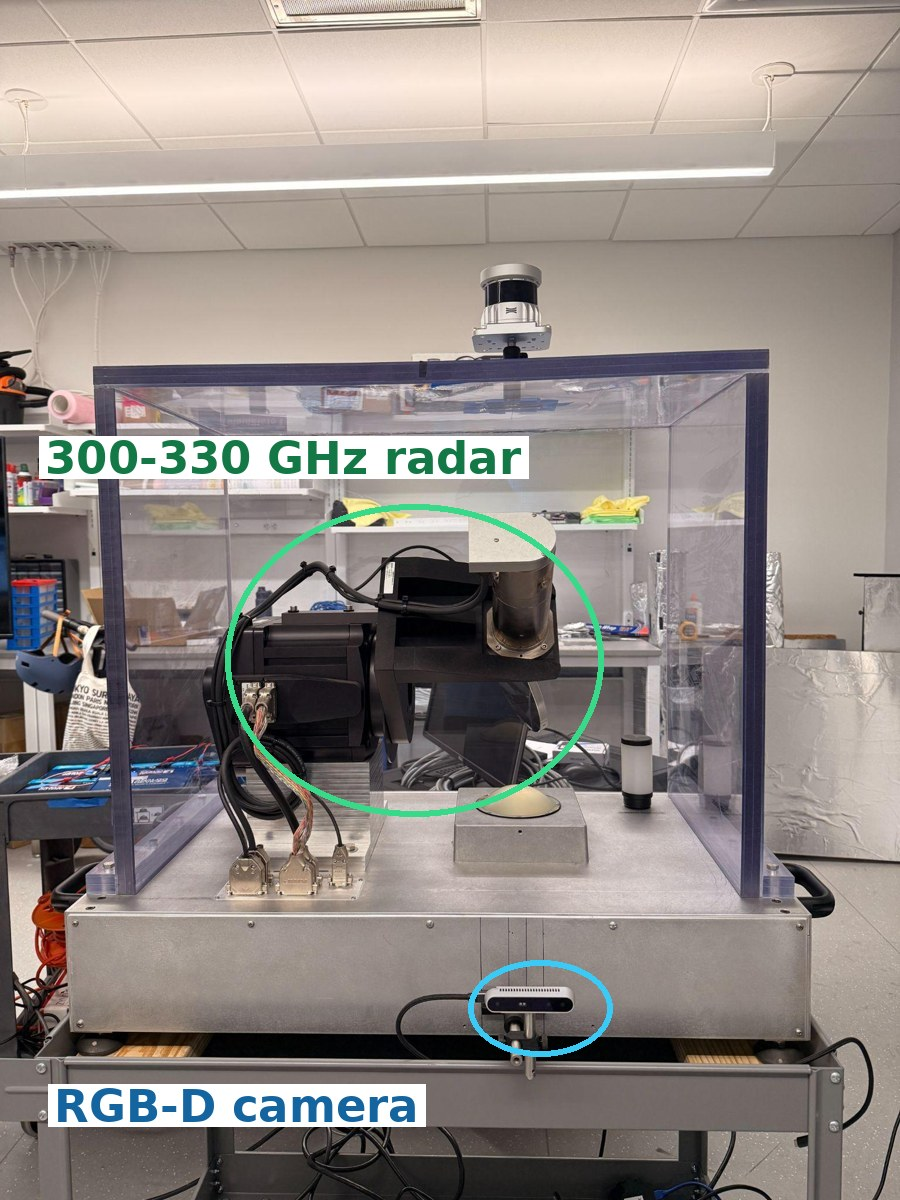
\includegraphics[width=0.62\columnwidth]{setup_annot.jpg}
\caption{Sensing system: the 300--330\,GHz imaging radar (green) and the RealSense D415 RGB-D camera (blue).}
\label{fig:setup}
\end{figure}

\subsection{Radar Point Cloud}
For each beam, the raw data are range-compressed with an FFT and the power is averaged over four scan passes. A range bin is detected when its power exceeds the median power of that beam by 25\,dB, and every local power peak among the detected bins becomes a point. Each detection is converted from (azimuth, elevation, range) to Cartesian coordinates and stored with its power in dB. A scan contains about 10{,}000 points.

\subsection{Body Crop and Automatic Labels}
Radar points are transformed into the camera frame and projected into the color image (Fig.~\ref{fig:label}). A point is kept as part of the body if it projects onto the mannequin mask from the depth image and lies between 10\,cm in front of and 45\,cm behind the RGB-D surface at that pixel. The window extends behind the surface because radar returns are smeared in depth by the coarse range resolution. Points less than 8\,cm above the floor or more than 45\,cm to either side of the body center are removed. For ground truth, the phone is found in the color image and its outline is grown by 4\,cm to allow for radar--camera misalignment. A body point is labeled \emph{phone} when it projects inside this outline and lies between 15\,cm in front of and 30\,cm behind the phone surface; the 30\,cm limit matches the range resolution.

\begin{figure}[t]
\centering
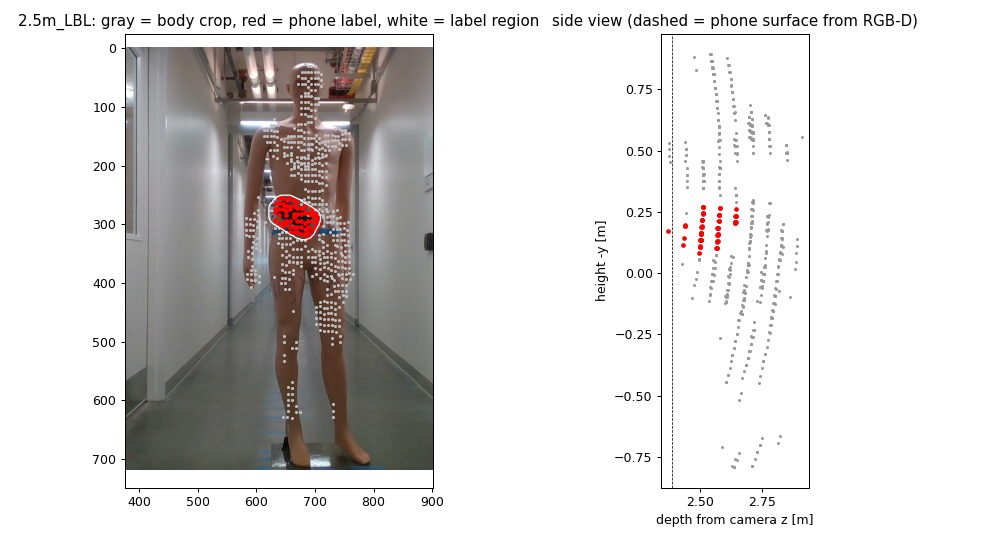
\includegraphics[width=\columnwidth]{label.png}
\caption{Automatic labeling. Left: radar points projected onto the color image; gray points are the body crop, red points are labeled phone, and the white contour is the grown phone outline. Right: side view, with the phone surface from the RGB-D camera dashed. Phone returns lie 5--27\,cm behind the surface.}
\label{fig:label}
\end{figure}

\subsection{Segmentation Model}
The network is trained on local patches rather than whole scans, which multiplies the number of training samples. Each patch is a 40$\times$40\,cm window extending $\pm$30\,cm in depth, from which 128 points are sampled. Each point has four features: its $x$, $y$, $z$ position relative to the patch center and its power relative to the median power of the scan, which removes the overall change in power with distance. PointNet++ uses four set-abstraction levels with neighborhood radii of 6, 10, 18 and 30\,cm, followed by four feature-propagation layers and a two-class output for every point. Because phone points are only about 14\% of the training points, the loss is a class-weighted negative log-likelihood. We train with Adam (learning rate $10^{-3}$) for 60 epochs of 2000 random patches, with batch size 32. Training patches are augmented with in-plane rotation up to $\pm45^\circ$, scaling, jitter and left--right mirroring, and thigh scans are sampled twice as often because they contain the fewest phone points. At test time the scan is covered by overlapping patches, the phone probability of each point is averaged over the patches that contain it, and points above 0.5 are labeled phone.

\subsection{Pilot Dataset and Metrics}
The pilot dataset contains 29 scans of a bare mannequin at 2.5, 3.0 and 3.5\,m: 26 scans with one phone taped on the left or right belly or thigh in four orientations, and 3 scans with no phone. The scans are split into 18 training, 4 validation and 7 test scans, with every distance in each split. We report the pooled phone IoU over all test points (correct phone points divided by correct, false and missed phone points), the detection rate (at least 3 predicted phone points within 10\,cm of the labeled phone), the fraction of scans with a false alarm (at least 3 predicted phone points elsewhere), and the error between the predicted and labeled phone centroids.

\section{Results (Partial)}
Within each scan, the median power of phone points was within about 1\,dB of the body on the belly and 4--7\,dB below it on the thighs. A power threshold therefore cannot separate the phone from the body, which motivates a model that uses local geometry.

Table~\ref{tab:results} and Fig.~\ref{fig:pred} summarize the test results. The model found all six test phones with a mean centroid error of 5.8\,cm, less than half a phone length. The pooled phone IoU was 0.34, and per-scan IoU ranged from 0.04 to 0.75. Belly phones were segmented best (0.75 at 2.5\,m and 0.46 at 3.5\,m), while thigh phones were found but only partly covered (0.10--0.30). Five of the seven test scans contained a false alarm, including 14 points on the scan with no phone.

\begin{table}[t]
\centering
\caption{PointNet++ results on the 7 held-out test scans}
\label{tab:results}
\begin{tabular}{lc}
\toprule
Metric & Value \\
\midrule
Pooled phone IoU & 0.34 \\
Per-scan IoU, belly (3 scans) & 0.04--0.75 \\
Per-scan IoU, thigh (3 scans) & 0.10--0.30 \\
Phones detected & 6 / 6 \\
Mean centroid error & 5.8\,cm \\
Scans with a false alarm & 5 / 7 \\
\bottomrule
\end{tabular}
\end{table}

\begin{figure}[t]
\centering
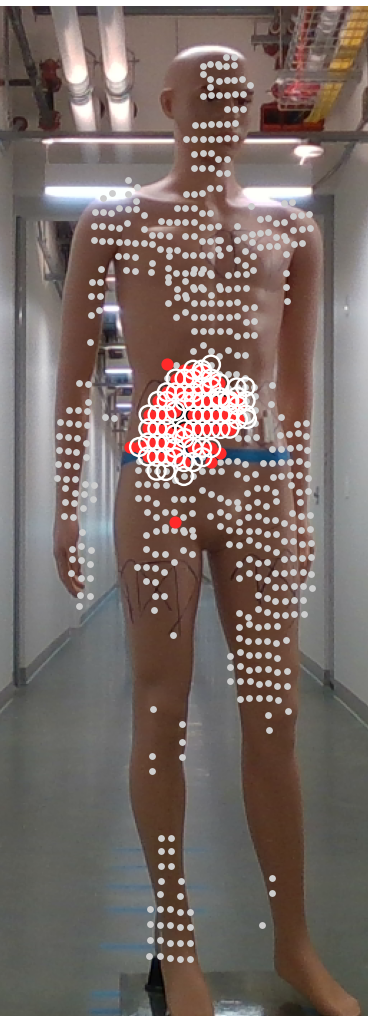
\includegraphics[height=1.75in]{pred_2p5m_LBR.png}\hfill
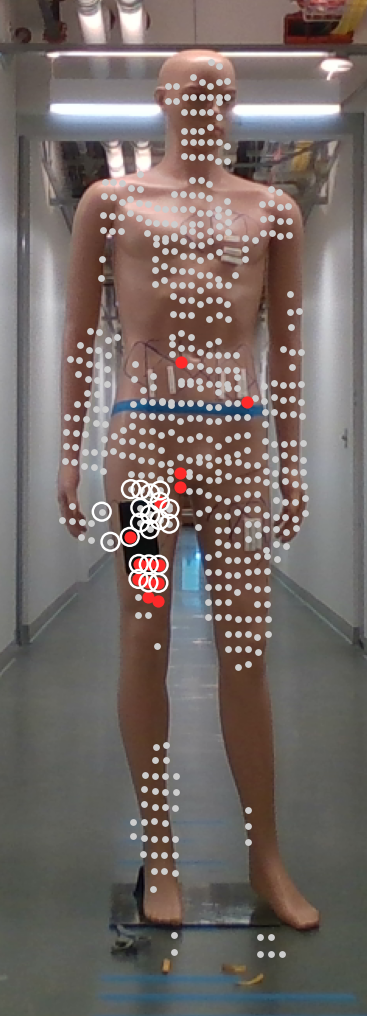
\includegraphics[height=1.75in]{pred_3p0m_LTM.png}\hfill
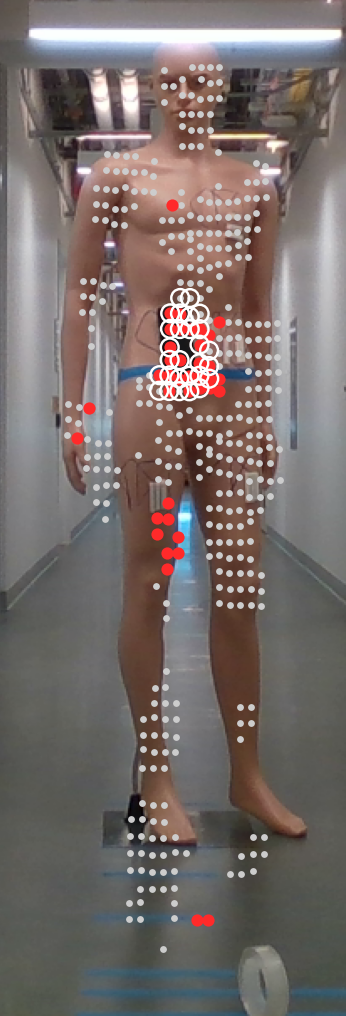
\includegraphics[height=1.75in]{pred_3p5m_LBM.png}\hfill
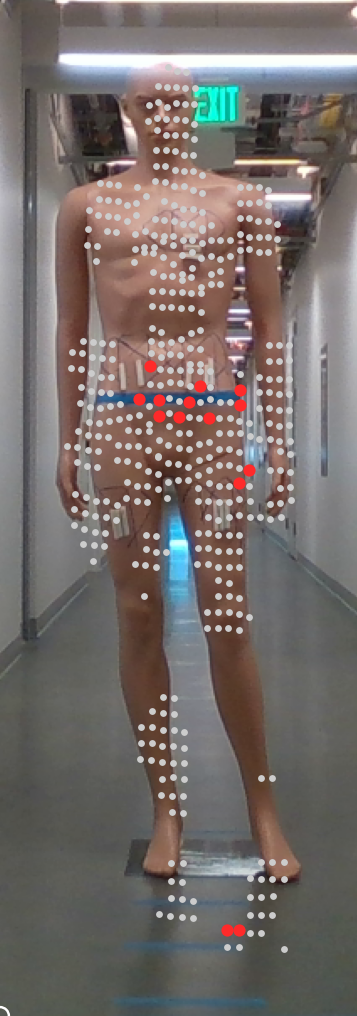
\includegraphics[height=1.75in]{pred_3p5m_bare.png}
\caption{Predictions on held-out scans; red points are predicted phone and white circles are the labels. From left: 2.5\,m belly (IoU 0.75), 3.0\,m thigh (0.30), 3.5\,m belly (0.46), and 3.5\,m with no phone, where false alarms appear near the waist.}
\label{fig:pred}
\end{figure}

\section{Discussion (Partial)}
The pilot shows that a point-set network can localize a phone on the body from radar points, even though the phone is not brighter than the body. Two weaknesses stand out. First, false alarms cluster around the waist. In the training data the belly phones always sit just above the waist, so the model partly associates the waist itself with a phone; more phone-free scans and scans with phones elsewhere are needed to break this link. Second, thigh phones are under-segmented because only five training scans have a phone on a thigh. We also found that two training runs differing only in a minor preprocessing step differed by about 0.05 in test IoU, so with only six test phones, differences of this size are not meaningful. Future comparisons will be averaged over several random seeds.

Next, we will collect scans with the mannequin dressed in three clothing types, with phones and everyday distractors such as keys, belts and card holders, labeled with the same pipeline. These data will be used to retrain the model and to evaluate tasks 2 and 3 against the targets stated in the Introduction.

\section*{Acknowledgements}
I thank Prof. Ashutosh Sabharwal for supervising this project, and Yiying Liu for mentorship and technical guidance on the radar system and data processing. I also thank the Rice Wireless Lab for access to the radar hardware and computing resources.

\section*{CRediT Author Statement}
% TODO: check each role and add your teammates' roles
\textbf{Yung-Hsin (Sean) Tsai:} Conceptualization, Methodology, Software, Investigation, Data curation, Formal analysis, Visualization, Writing -- original draft.\\

\begin{thebibliography}{00}
\bibitem{sheen2001} D.~M. Sheen, D.~L. McMakin, and T.~E. Hall, ``Three-dimensional millimeter-wave imaging for concealed weapon detection,'' \textit{IEEE Trans. Microw. Theory Techn.}, vol.~49, no.~9, pp.~1581--1592, Sep. 2001.
\bibitem{meng2020} Z. Meng, M. Zhang, and H. Wang, ``CNN with pose segmentation for suspicious object detection in MMW security images,'' \textit{Sensors}, vol.~20, no.~17, Art. no.~4974, 2020.
\bibitem{pang2020} L. Pang, H. Liu, Y. Chen, and J. Miao, ``Real-time concealed object detection from passive millimeter wave images based on the YOLOv3 algorithm,'' \textit{Sensors}, vol.~20, no.~6, Art. no.~1678, 2020.
\bibitem{mitchell2023} K. Mitchell, K. Kassem, C. Kaul, V. Kapitany, P. Binner, A. Ramsay, D. Faccio, and R. Murray-Smith, ``mmSense: Detecting concealed weapons with a miniature radar sensor,'' in \textit{Proc. IEEE Int. Conf. Acoust., Speech Signal Process. (ICASSP)}, Rhodes, Greece, 2023, doi: 10.1109/ICASSP49357.2023.10095884.
\bibitem{kaul2024} C. Kaul, K.~J. Mitchell, K. Kassem, A. Tragakis, V. Kapitany, I. Starshynov, F. Villa, R. Murray-Smith, and D. Faccio, ``AI-enabled sensor fusion of time-of-flight imaging and mmWave for concealed metal detection,'' \textit{Sensors}, vol.~24, no.~18, Art. no.~5865, 2024.
\bibitem{qi2017pointnet} C.~R. Qi, H. Su, K. Mo, and L.~J. Guibas, ``PointNet: Deep learning on point sets for 3D classification and segmentation,'' in \textit{Proc. IEEE Conf. Comput. Vis. Pattern Recognit. (CVPR)}, 2017, pp.~652--660.
\bibitem{qi2017pointnetpp} C.~R. Qi, L. Yi, H. Su, and L.~J. Guibas, ``PointNet++: Deep hierarchical feature learning on point sets in a metric space,'' in \textit{Proc. Adv. Neural Inf. Process. Syst. (NeurIPS)}, 2017, pp.~5099--5108.
\end{thebibliography}

\end{document}
